\begin{columns}
  \begin{column}{0.17\linewidth}
    
\includegraphics[width=0.5\linewidth]{kth_cmyk.eps}
    \hfill
  \end{column}
  \hfill
  \begin{column}{0.64\linewidth}
    \begin{center}
      \Huge\bfseries
      Securely and Privately Verifiable Protests
    \end{center}
    \begin{center}
      \large
      Daniel Bosk <dbosk@kth.se>
      $\bullet$
      Sonja Buchegger
      $\bullet$
      Sébastien Gambs
    \end{center}
    \vspace{1.5em}
  \end{column}
  \hfill
  \begin{column}{0.17\linewidth}
    \hfill
    
\includegraphics[width=0.8\linewidth]{uqam.pdf}
  \end{column}
\end{columns}

\vfill

\includegraphics[width=\linewidth]{ProtestVerif.png}

\vfill

\begin{columns}[t]

  \begin{column}{0.32\linewidth}

    \begin{redblock}{Verifying protest participation}
      \begin{itemize}
        \item Alice wants to show that many support her cause.
        \item Eve wants to show that few support Alice's cause.
        \item {\color{red} Adversarial setting, requires verifiable results!}
          (E.g.\ \cref{TrumpInauguration}.)
      \end{itemize}
    \end{redblock}

    \begin{blueblock}{Requirements for verifiability}
      \begin{itemize}
        \item\label{EligibilityVerif} Eligibility: anyone can verify that each 
          participation proof provides temporal and spatial eligibility and that 
          it has not been counted before.

        \item\label{UniversalVerif} Universal verifiability: anyone can verify 
          that the result is according to the submitted participation proofs.

        \item\label{IndividualVerif} Individual verifiability: every participant 
          can verify that their participation proof is included in the global 
          count.
      \end{itemize}
    \end{blueblock}

    \begin{blueblock}{Requirements for privacy}
      \begin{itemize}
        \item Protocol should not harm the privacy of the protester, i.e.\  not 
          diclose any information about them other than what can already be 
          learnt from their physical attendance.
      \end{itemize}
    \end{blueblock}

  \end{column}

  \hfill

  \begin{column}{0.32\linewidth}

    \begin{figure}
      \centering
      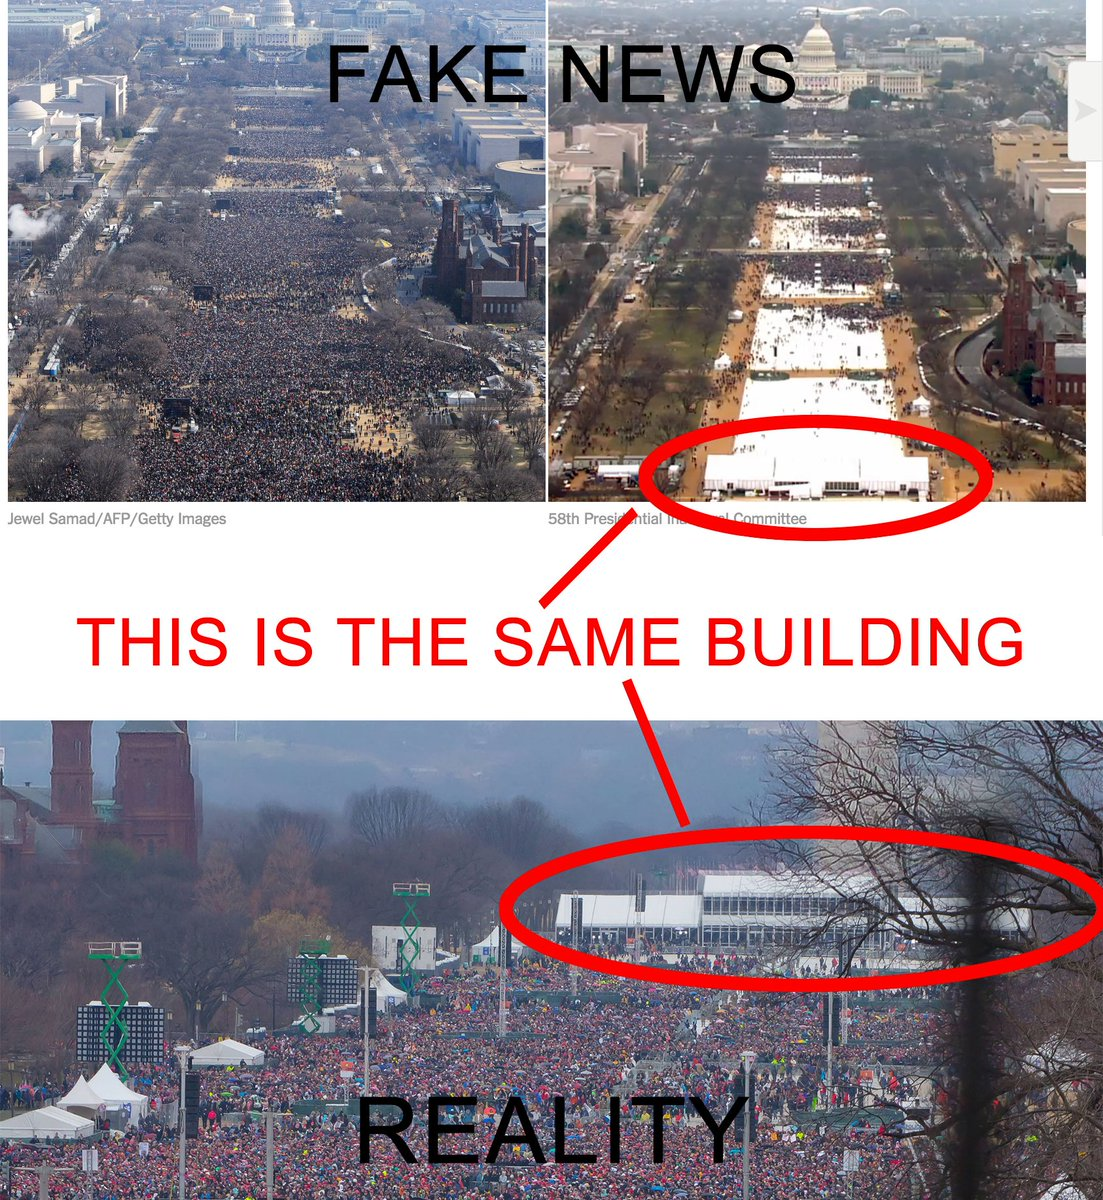
\includegraphics[width=0.9\linewidth]{trump.jpg}
      \caption{%
        What can we trust?
        This picture was posted on Twitter (and linked from Reddit) to argue 
        that the news reporting on the participation count was \enquote{fake 
          news} and that Trump's supporters arrived later.
        Even if the picture labelled \enquote{REALITY} would be from the same 
        event (difficult to verify), it is difficult to accurately compare due 
        to the angle.
        Image: Reddit/The\_Donald, Twitter.
      }\label{TrumpInauguration}
    \end{figure}

  \end{column}

  \hfill

  \begin{column}{0.32\linewidth}

    \begin{greenblock}{Our approach}
      \begin{itemize}
        \item Provides a \emph{lower bound} of the participation count.
        \item This lower bound is cryptographically verifiable.
        \item Provides privacy based on anonymous credentials and 
          privacy-preserving proximity testing.
        \item The only added risk (over not using this) is if someone can use 
          your secret key.
        \item Requires only local connectivity during the protest.
        \item Requires no trust in the source (as in \cref{TrumpInauguration}), 
          only that IDs are issued correctly.
      \end{itemize}
    \end{greenblock}

    \includegraphics[width=\linewidth]{ProtestVerif-UN.png}

  \end{column}

\end{columns}

\vfill

\begin{columns}[t]

  \begin{column}{0.32\linewidth}

    \begin{figure}
      \centering
      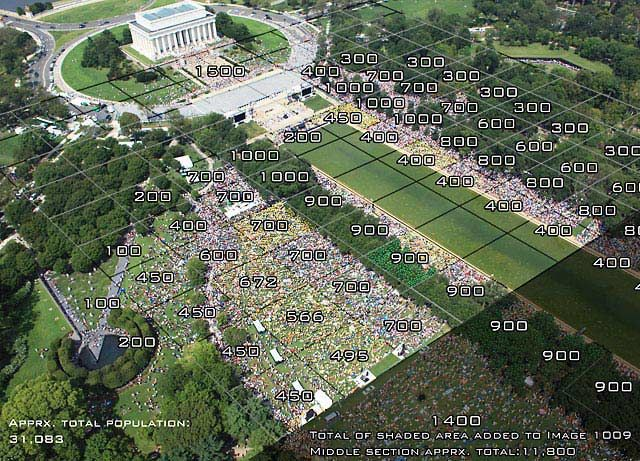
\includegraphics[width=\linewidth]{Jacobs-method.jpg}
      \caption{%
        Jacobs Method, currently most used method.
        Divide into regions, estimate density in each region, sum up.
        Image: popularmechanics.com
      }\label{JacobsMethod}
    \end{figure}

    \begin{purpleblock}{Current crowd-counting methods}
      \begin{itemize}
        \item Most used method, Jacobs Method (\cref{JacobsMethod}).
        \item {\color{red} Cannot handle cumulative counts, faces problems 
            illustrated by \cref{TrumpInauguration}.}
        \item Computer vision does object recognition; requires photos/video 
          that cover the entire location, all the time.
        \item {\color{red} This will still count people twice.}
        \item Scan active mobile phones (or similar) in the area.
        \item This requires some extra equipment.
        \item {\color{red} This catches bystanders who are not protesting.}
        \item {\color{red} Neither method can distinguish two close but 
            different protests (e.g.\ pro- and anti-protests).}
      \end{itemize}
    \end{purpleblock}

  \end{column}

  \hfill

  \begin{column}{0.32\linewidth}

    \begin{blackblock}{Our scheme, during protest (\cref{ProofShare}, top of 
        \cref{Protocol})}
      \begin{itemize}
        \item The organizer publishes the protest's manifesto.
        \item Each protester reads it, approves it, computes a protest (cause) 
          identifier (\(cid\)) to designate which protest they participate in.
        \item Each protester computes a personal identifier (\(pid\)), 
          unlinkable between protests,
        \item Each protester acts as witness (\(wid\), unlinkable between 
          protesters, \(wsig\)) for other protesters by creating 
          participation-proof shares.
        \item Proof shares vouches for temporal and spatial eligibility.
        \item A threshold-based number of valid shares is a valid proof.
      \end{itemize}
    \end{blackblock}

    \begin{blackblock}{Our scheme, after the protest (bottom of 
        \cref{Protocol})}
      \begin{itemize}
        \item Proof shares are committed to a blockchain as soon as possible.
        \item \Ac{NIZK} proofs of correctness of \(PRF\) computations and 
          validity of keys are submitted whenever convenient.
        \item Anyone can verify the proofs: eligibility, universal and 
          individual verifiability.
        \item Must be done for all shares and their \ac{NIZK} proofs.
        \item Count all \(pid\)s with valid proofs.
      \end{itemize}
    \end{blackblock}

    \begin{block}{More info}
      \centering
      \includegraphics[width=0.4\linewidth]{qr.eps}
    \end{block}

    \printbibliography[heading=none]

  \end{column}

  \hfill

  \begin{column}{0.32\linewidth}
    \begin{figure}
      \centering
      \includegraphics[width=\linewidth]{proofshare.tikz}
      \caption{%
        Structure of a proof share.
        The protester \(P\)'s identifier \(pid\) is computed using the protester's 
        key \(k_P\).
        The witness \(W\)'s identifier \(wid\) is computed using the witness's key 
        \(k_W\).
        \(t_s\) is a time interval and \(l\) is the coordinates of an area.
        The protest (cause) identifier \(cid\) is the hash value of the manifesto.
      }%
      \label{ProofShare}
    \end{figure}%

    \begin{figure}
      \centering
      \begin{minipage}{\linewidth}
        \begin{align*}
          O\to \text{all}\colon & \text{manifesto} \\
          P\colon & cid\gets H(\text{manifesto}), \\
          & pid\gets PRF_{k_P}(cid) \\
          P\to W\colon & pid \\
          W\leftrightarrow P\colon & \text{perform distance bounding} \\
          W\colon & wid\gets PRF_{k_W}(pid), \\
          & wsig\gets PRF_{k_W}(wid, t_s, l) \\
          W\to P\colon & (wid, t_s, l, wsig) \\[-1em]
          && \text{during protest} \\ \midrule && \text{after protest} \\[-1em]
          W\to S\colon & H(pid, wid, t_s, l, wsig) \\
          P\to S\colon & H(pid, wid, t_s, l, wsig) \\
          W\to S\colon & (pid, wid, t_s, l, wsig),\\
          & NIZK( wid = PRF_{k_W}(pid), \\
          & wsig = PRF_{k_W}(wid, t_s, l), \\
          & \exists sign(k_W)) \\
          P\to S\colon & (pid, wid, t_s, l, wsig),\\
          & NIZK(pid = PRF_{k_P}(cid), \exists sign(k_P))
        \end{align*}
      \end{minipage}
      \caption{%
        An overview of message exchanges.
        The organizer \(O\) broadcasts the manifesto.
        \(P\), \(W\) and their computations are as in \cref{ProofShare}.
        Finally, both \(P\) and \(W\) submits the proof share to the storage \(S\).
      }%
      \label{Protocol}
    \end{figure}

  \end{column}

\end{columns}

\vfill
\flushright{}
Special thanks to xkcd.com which, over many years, has inspired the stylistic 
presentation of this poster.
